\begin{figure}[h]
\begin{subfigure}{0.3\textwidth}
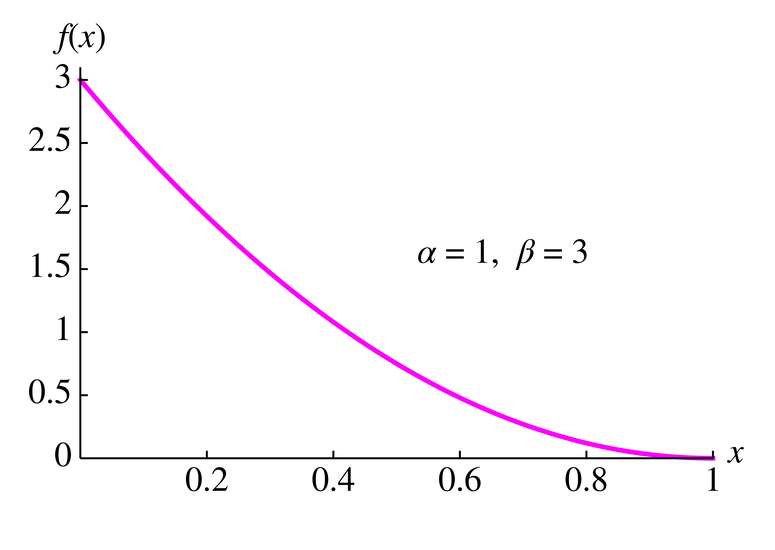
\includegraphics[width=0.3\linewidth]{beta.png}
\caption{beta}
\end{subfigure}
\begin{subfigure}{0.3\textwidth}
    \includegraphics[width=0.3\linewidth]{binominal.png}
    \caption{binominal}
\end{subfigure}
\begin{subfigure}{0.3\textwidth}
    \includegraphics[width=0.3\linewidth]{epsilon_lambda.png}
    \caption{epsilon lambda}
\end{subfigure}
\end{figure}
\begin{figure}[h]
\begin{subfigure}{0.3\textwidth}
    \includegraphics[width=0.3\linewidth]{gama.png}
    \caption{gama}
\end{subfigure}
\begin{subfigure}{0.3\textwidth}
    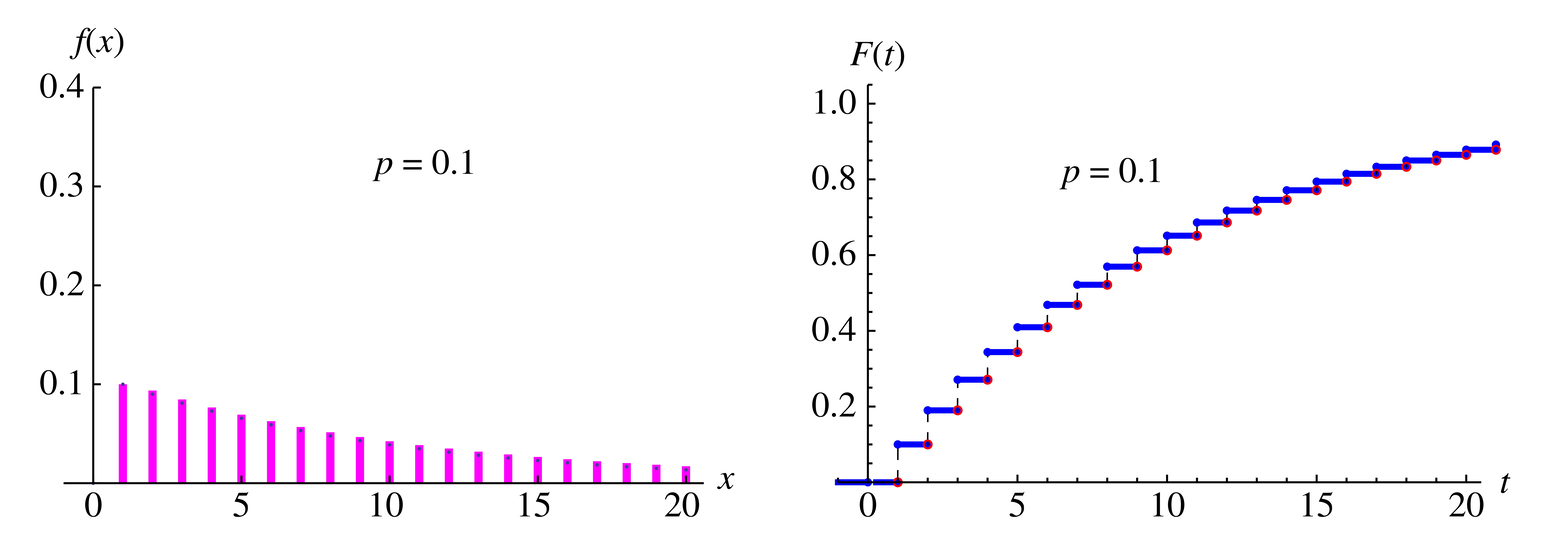
\includegraphics[width=0.3\linewidth]{geom.png}
    \caption{geom}
\end{subfigure}
\begin{subfigure}{0.3\textwidth}
    \includegraphics[width=0.3\linewidth]{hyperg.png}
    \caption{hyperg}
\end{subfigure}
\end{figure}
\begin{figure}[h]
\begin{subfigure}{0.3\textwidth}
    \includegraphics[width=0.3\linewidth]{normal.png}
    \caption{normal}
\end{subfigure}
\begin{subfigure}{0.3\textwidth}
    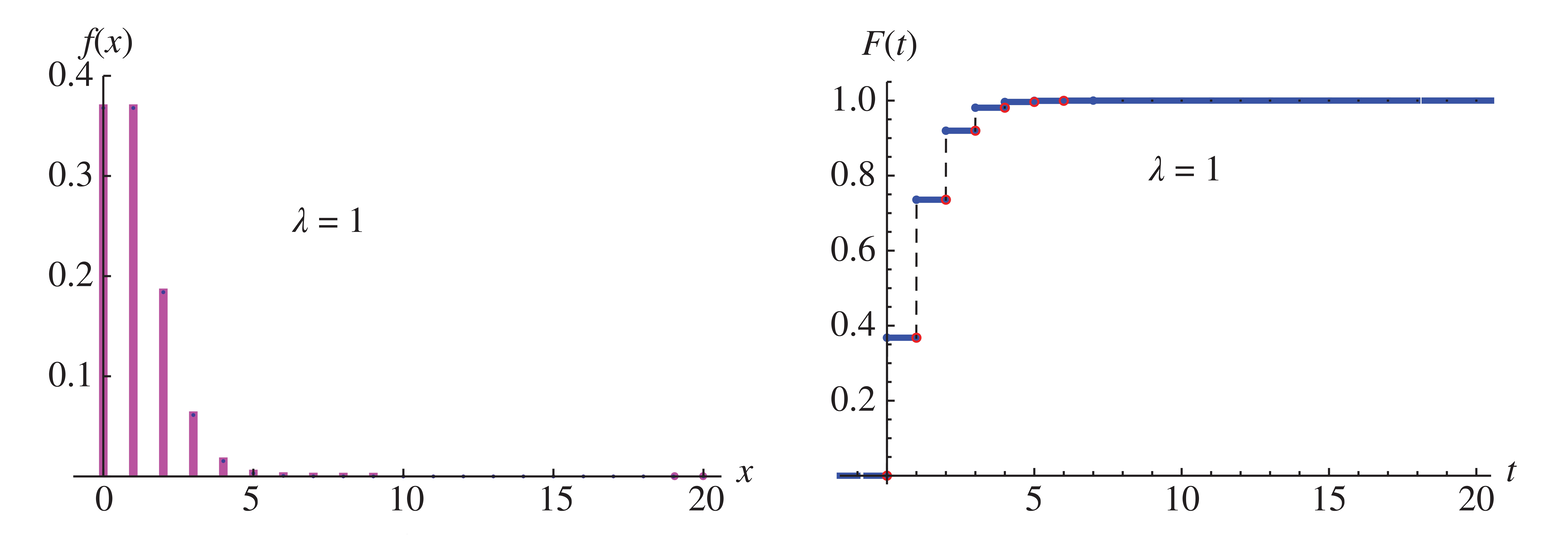
\includegraphics[width=0.3\linewidth]{poisson.png}
    \caption{poisson}
\end{subfigure}
\begin{subfigure}{0.3\textwidth}
    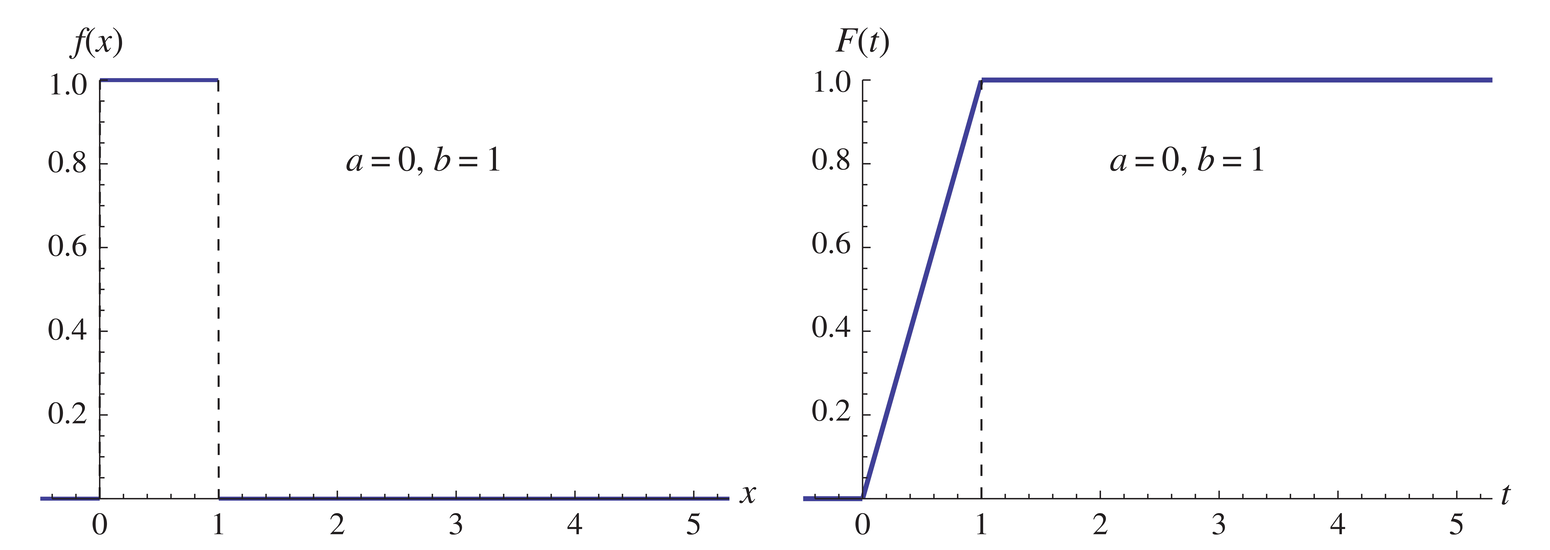
\includegraphics[width=0.3\linewidth]{uniforme.png}
    \caption{uniforme}
\end{subfigure}
\end{figure}